\documentclass[a4paper]{book}
\usepackage{a4wide}
\usepackage{makeidx}
\usepackage{graphicx}
\usepackage{multicol}
\usepackage{float}
\usepackage{listings}
\usepackage{color}
\usepackage{textcomp}
\usepackage{alltt}
\usepackage{times}
\usepackage{ifpdf}
\ifpdf
\usepackage[pdftex,
            pagebackref=true,
            colorlinks=true,
            linkcolor=blue,
            unicode
           ]{hyperref}
\else
\usepackage[ps2pdf,
            pagebackref=true,
            colorlinks=true,
            linkcolor=blue,
            unicode
           ]{hyperref}
\usepackage{pspicture}
\fi
\usepackage[utf8]{inputenc}
\usepackage{doxygen}
\lstset{language=C++,inputencoding=utf8,basicstyle=\footnotesize,breaklines=true,breakatwhitespace=true,tabsize=2,numbers=left }
\makeindex
\setcounter{tocdepth}{3}
\renewcommand{\footrulewidth}{0.4pt}
\begin{document}
\hypersetup{pageanchor=false}
\begin{titlepage}
\vspace*{7cm}
\begin{center}
{\Large phpVC \\[1ex]\large 1 }\\
\vspace*{1cm}
{\large Generated by Doxygen 1.7.1}\\
\vspace*{0.5cm}
{\small Mon Aug 30 2010 18:19:55}\\
\end{center}
\end{titlepage}
\clearemptydoublepage
\pagenumbering{roman}
\tableofcontents
\clearemptydoublepage
\pagenumbering{arabic}
\hypersetup{pageanchor=true}
\chapter{Data Structure Index}
\section{Class Hierarchy}
This inheritance list is sorted roughly, but not completely, alphabetically:\begin{DoxyCompactList}
\item \contentsline{section}{Controller}{\pageref{class_controller}}{}
\begin{DoxyCompactList}
\item \contentsline{section}{TestController}{\pageref{class_test_controller}}{}
\end{DoxyCompactList}
\item \contentsline{section}{Database}{\pageref{class_database}}{}
\item \contentsline{section}{Dispatcher}{\pageref{class_dispatcher}}{}
\end{DoxyCompactList}

\chapter{Data Structure Index}
\section{Data Structures}
Here are the data structures with brief descriptions:\begin{DoxyCompactList}
\item\contentsline{section}{\hyperlink{class_controller}{Controller} (Defines \hyperlink{class_controller}{Controller} class )}{\pageref{class_controller}}{}
\item\contentsline{section}{\hyperlink{class_database}{Database} (Defines Database(), an interface object providing access to the database )}{\pageref{class_database}}{}
\item\contentsline{section}{\hyperlink{class_dispatcher}{Dispatcher} (Parses the url and invokes the correct controller )}{\pageref{class_dispatcher}}{}
\item\contentsline{section}{\hyperlink{class_test_controller}{TestController} (Typical controller derives from \hyperlink{class_controller}{Controller} )}{\pageref{class_test_controller}}{}
\end{DoxyCompactList}

\chapter{File Index}
\section{File List}
Here is a list of all files with brief descriptions:\begin{DoxyCompactList}
\item\contentsline{section}{C:/AppServ/www/book/\hyperlink{controller_8php}{controller.php} }{\pageref{controller_8php}}{}
\item\contentsline{section}{C:/AppServ/www/book/\hyperlink{db_8php}{db.php} }{\pageref{db_8php}}{}
\item\contentsline{section}{C:/AppServ/www/book/\hyperlink{dispatch_8php}{dispatch.php} }{\pageref{dispatch_8php}}{}
\item\contentsline{section}{C:/AppServ/www/book/\hyperlink{index_8php}{index.php} }{\pageref{index_8php}}{}
\item\contentsline{section}{C:/AppServ/www/book/\hyperlink{passwd_8php}{passwd.php} }{\pageref{passwd_8php}}{}
\item\contentsline{section}{C:/AppServ/www/book/controllers/\hyperlink{test__controller_8php}{test\_\-controller.php} }{\pageref{test__controller_8php}}{}
\item\contentsline{section}{C:/AppServ/www/book/views/layouts/\hyperlink{test_8php}{test.php} }{\pageref{test_8php}}{}
\item\contentsline{section}{C:/AppServ/www/book/views/test/\hyperlink{page_8php}{page.php} }{\pageref{page_8php}}{}
\end{DoxyCompactList}

\chapter{Data Structure Documentation}
\hypertarget{class_controller}{
\section{Controller Class Reference}
\label{class_controller}\index{Controller@{Controller}}
}


Defines \hyperlink{class_controller}{Controller} class.  


Inheritance diagram for Controller:\begin{figure}[H]
\begin{center}
\leavevmode
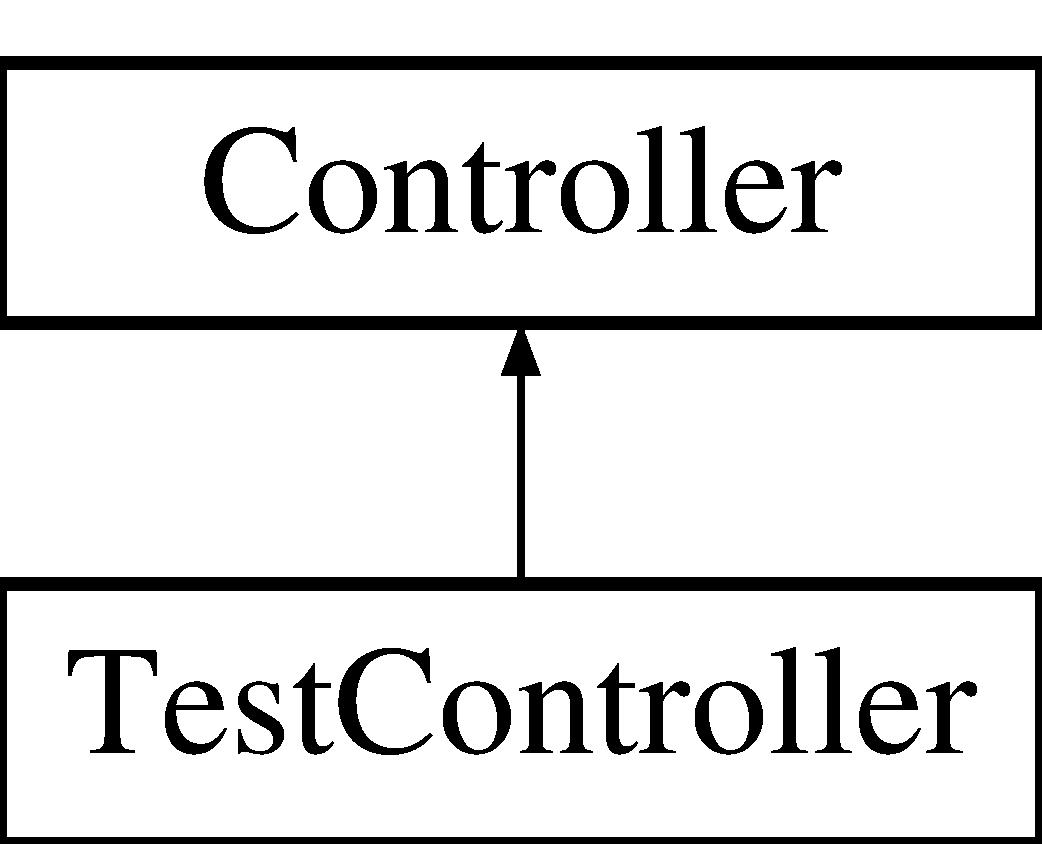
\includegraphics[height=2.000000cm]{class_controller}
\end{center}
\end{figure}
\subsection*{Static Public Member Functions}
\begin{DoxyCompactItemize}
\item 
static \hyperlink{class_controller_a5b07b6865d0d974cd0e7198affae054f}{render} (\$controller, \$action, \$params=NULL)
\begin{DoxyCompactList}\small\item\em renders a view of the specific action, with the layout for the specific controller. \item\end{DoxyCompactList}\item 
static \hyperlink{class_controller_a6d111024445bc17d76a64b45f49d2d69}{redirect} (\$url, \$\_\-get=NULL)
\begin{DoxyCompactList}\small\item\em redirect to a specific url, which will invoke the controller method call \item\end{DoxyCompactList}\item 
static \hyperlink{class_controller_a18b050608bad4c25d29425778c76af49}{path\_\-to} (\$controller, \$action, \$\_\-get=NULL)
\begin{DoxyCompactList}\small\item\em returns a string representing an URL path pointing to an action \item\end{DoxyCompactList}\item 
static \hyperlink{class_controller_a86600c0af25bc98587b49950b3ae4408}{stylesheet\_\-link\_\-tag} (\$file\_\-name)
\begin{DoxyCompactList}\small\item\em returns a string of a link tag \item\end{DoxyCompactList}\item 
static \hyperlink{class_controller_a6732e0005a1160d36b0287eb95204755}{javascript\_\-include\_\-tag} (\$file\_\-name)
\begin{DoxyCompactList}\small\item\em returns a string of a script tag \item\end{DoxyCompactList}\end{DoxyCompactItemize}


\subsection{Detailed Description}
Defines \hyperlink{class_controller}{Controller} class. \hyperlink{class_controller}{Controller} provides common static methods such as render the views, redirect to another url and some helper functions that helps with the view. \hyperlink{class_controller}{Controller} class will be inherited by other controllers. Inherited controllers, or Derived controllers, must follow the naming rule of \{Controllername\}\hyperlink{class_controller}{Controller}, for example, UserController. the name of the controller is followed by the word 'Controller' with the first letter capitalized. Notice that in PHP, class names are case-\/sensitive. 

Definition at line 16 of file controller.php.



\subsection{Member Function Documentation}
\hypertarget{class_controller_a6732e0005a1160d36b0287eb95204755}{
\index{Controller@{Controller}!javascript\_\-include\_\-tag@{javascript\_\-include\_\-tag}}
\index{javascript\_\-include\_\-tag@{javascript\_\-include\_\-tag}!Controller@{Controller}}
\subsubsection[{javascript\_\-include\_\-tag}]{\setlength{\rightskip}{0pt plus 5cm}static javascript\_\-include\_\-tag (
\begin{DoxyParamCaption}
\item[{\$}]{ file\_\-name}
\end{DoxyParamCaption}
)\hspace{0.3cm}{\ttfamily  \mbox{[}static\mbox{]}}}}
\label{class_controller_a6732e0005a1160d36b0287eb95204755}


returns a string of a script tag 



Definition at line 94 of file controller.php.




\begin{DoxyCode}
                                                           {
    $script_path = substr($_SERVER['SCRIPT_NAME'], 0, strrpos($_SERVER['SCRIPT_NA
      ME'], '/')+1);
    srand(); $salt = rand();
    return "<script type=\"text/javascript\" src=\"$script_path$file_name?$salt\"
      ></script>\n";
  }
\end{DoxyCode}


\hypertarget{class_controller_a18b050608bad4c25d29425778c76af49}{
\index{Controller@{Controller}!path\_\-to@{path\_\-to}}
\index{path\_\-to@{path\_\-to}!Controller@{Controller}}
\subsubsection[{path\_\-to}]{\setlength{\rightskip}{0pt plus 5cm}static path\_\-to (
\begin{DoxyParamCaption}
\item[{\$}]{ controller, }
\item[{\$}]{ action, }
\item[{\$}]{ \_\-get = {\ttfamily NULL}}
\end{DoxyParamCaption}
)\hspace{0.3cm}{\ttfamily  \mbox{[}static\mbox{]}}}}
\label{class_controller_a18b050608bad4c25d29425778c76af49}


returns a string representing an URL path pointing to an action 


\begin{DoxyParams}{Parameters}
\item[{\em \$controller}]controller name \item[{\em \$action}]action name \item[{\em \$\_\-get}]the \$\_\-GET\mbox{[}\mbox{]} array to attach on the layout \end{DoxyParams}


Definition at line 78 of file controller.php.




\begin{DoxyCode}
                                                                  {
    $script_path = substr($_SERVER['SCRIPT_NAME'], 0, strrpos($_SERVER['SCRIPT_NA
      ME'], '/')+1);
    if(is_array($_get))
      return $script_path.$controller.'/'.$action.'?'.http_build_query($_get);
    else
      return $script_path.$controller.'/'.$action;
  }
\end{DoxyCode}


\hypertarget{class_controller_a6d111024445bc17d76a64b45f49d2d69}{
\index{Controller@{Controller}!redirect@{redirect}}
\index{redirect@{redirect}!Controller@{Controller}}
\subsubsection[{redirect}]{\setlength{\rightskip}{0pt plus 5cm}static redirect (
\begin{DoxyParamCaption}
\item[{\$}]{ url, }
\item[{\$}]{ \_\-get = {\ttfamily NULL}}
\end{DoxyParamCaption}
)\hspace{0.3cm}{\ttfamily  \mbox{[}static\mbox{]}}}}
\label{class_controller_a6d111024445bc17d76a64b45f49d2d69}


redirect to a specific url, which will invoke the controller method call 


\begin{DoxyParams}{Parameters}
\item[{\em \$url}]an url like login/index \item[{\em \$\_\-get}]the \$\_\-GET\mbox{[}\mbox{]} array to attach on the layout \end{DoxyParams}


Definition at line 58 of file controller.php.




\begin{DoxyCode}
                                                   {
    $script_path = substr($_SERVER['SCRIPT_NAME'], 0, strrpos($_SERVER['SCRIPT_NA
      ME'], '/')+1);
    
    if(is_array($_get))
      header( "location: $script_path$url?".http_build_query($_get) );
    else
      header( "location: $script_path$url" );
      
    exit(0);
  }
\end{DoxyCode}


\hypertarget{class_controller_a5b07b6865d0d974cd0e7198affae054f}{
\index{Controller@{Controller}!render@{render}}
\index{render@{render}!Controller@{Controller}}
\subsubsection[{render}]{\setlength{\rightskip}{0pt plus 5cm}static render (
\begin{DoxyParamCaption}
\item[{\$}]{ controller, }
\item[{\$}]{ action, }
\item[{\$}]{ params = {\ttfamily NULL}}
\end{DoxyParamCaption}
)\hspace{0.3cm}{\ttfamily  \mbox{[}static\mbox{]}}}}
\label{class_controller_a5b07b6865d0d974cd0e7198affae054f}


renders a view of the specific action, with the layout for the specific controller. 


\begin{DoxyParams}{Parameters}
\item[{\em \$controller}]layout to use \item[{\em \$action}]view to put in layout \item[{\em \$params}]params passed into the layout and the view \end{DoxyParams}


\$\_\-\_\-script\_\-path specifies the current script path (to the root of the app). It can be used inside views and layouts.

A layout should contain \char`\"{}require(\$\_\-\_\-view\_\-\_\-);\char`\"{} to call the view. 



Definition at line 32 of file controller.php.




\begin{DoxyCode}
                                                                   {
    $__script_path = substr($_SERVER['SCRIPT_NAME'], 0, strrpos($_SERVER['SCRIPT_
      NAME'], '/')+1); 
    $__view__ = "views/$controller/$action.php";

    if(!file_exists("views/layouts/$controller.php")){ // a controller without la
      yout
      if(!file_exists($__view__))
        self::error($controller, $action, "$__view__ does not exist.");
        require($__view__);       // directly includes the view
        // $params can be used within the layout and view.
    }else{
      // include the layout
      require("views/layouts/$controller.php");
      
      // $params can be used within the layout and view.
    }
    exit(0);
  }
\end{DoxyCode}


\hypertarget{class_controller_a86600c0af25bc98587b49950b3ae4408}{
\index{Controller@{Controller}!stylesheet\_\-link\_\-tag@{stylesheet\_\-link\_\-tag}}
\index{stylesheet\_\-link\_\-tag@{stylesheet\_\-link\_\-tag}!Controller@{Controller}}
\subsubsection[{stylesheet\_\-link\_\-tag}]{\setlength{\rightskip}{0pt plus 5cm}static stylesheet\_\-link\_\-tag (
\begin{DoxyParamCaption}
\item[{\$}]{ file\_\-name}
\end{DoxyParamCaption}
)\hspace{0.3cm}{\ttfamily  \mbox{[}static\mbox{]}}}}
\label{class_controller_a86600c0af25bc98587b49950b3ae4408}


returns a string of a link tag 



Definition at line 87 of file controller.php.




\begin{DoxyCode}
                                                        {
    $script_path = substr($_SERVER['SCRIPT_NAME'], 0, strrpos($_SERVER['SCRIPT_NA
      ME'], '/')+1);
    srand(); $salt = rand();
    return "<link href=\"$script_path$file_name?$salt\" rel=\"stylesheet\" type=\
      "text/css\" />\n";
  }
\end{DoxyCode}




The documentation for this class was generated from the following file:\begin{DoxyCompactItemize}
\item 
C:/AppServ/www/book/\hyperlink{controller_8php}{controller.php}\end{DoxyCompactItemize}

\hypertarget{class_database}{
\section{Database Class Reference}
\label{class_database}\index{Database@{Database}}
}


defines Database(), an interface object providing access to the database.  


\subsection*{Public Member Functions}
\begin{DoxyCompactItemize}
\item 
\hyperlink{class_database_a095c5d389db211932136b53f25f39685}{\_\-\_\-construct} ()
\begin{DoxyCompactList}\small\item\em connect to the database when an instance of \hyperlink{class_database}{Database} is created. \item\end{DoxyCompactList}\item 
\hyperlink{class_database_a421831a265621325e1fdd19aace0c758}{\_\-\_\-destruct} ()
\begin{DoxyCompactList}\small\item\em close the database connection when an instance of \hyperlink{class_database}{Database} destroied. \item\end{DoxyCompactList}\item 
\hyperlink{class_database_adcf17a809c87f756d7645da0483e9362}{getArr} (\$sql, \$index\_\-column= '')
\begin{DoxyCompactList}\small\item\em return row result as a 2-\/D array. \item\end{DoxyCompactList}\item 
\hyperlink{class_database_ac9fddec3f6bd1db128887a1b211d90f0}{query} (\$query)
\begin{DoxyCompactList}\small\item\em sends a query to the database \item\end{DoxyCompactList}\item 
\hyperlink{class_database_adda9fb830c1f42c98e409084d5e765b7}{getInsertId} ()
\begin{DoxyCompactList}\small\item\em returns the last inserted id. \item\end{DoxyCompactList}\item 
\hyperlink{class_database_a7b8701a38c6f1b80fd0659bfda3a68f7}{escape} (\$text)
\begin{DoxyCompactList}\small\item\em returns a sanitized string that is ready to be inserted to the SQL command. \item\end{DoxyCompactList}\end{DoxyCompactItemize}
\subsection*{Data Fields}
\begin{DoxyCompactItemize}
\item 
const \hyperlink{class_database_a758c150b67e476ecf77478f16b387c61}{DEBUG} = true
\end{DoxyCompactItemize}


\subsection{Detailed Description}
defines Database(), an interface object providing access to the database. 

Definition at line 5 of file db.php.



\subsection{Constructor \& Destructor Documentation}
\hypertarget{class_database_a095c5d389db211932136b53f25f39685}{
\index{Database@{Database}!\_\-\_\-construct@{\_\-\_\-construct}}
\index{\_\-\_\-construct@{\_\-\_\-construct}!Database@{Database}}
\subsubsection[{\_\-\_\-construct}]{\setlength{\rightskip}{0pt plus 5cm}\_\-\_\-construct (
\begin{DoxyParamCaption}
{}
\end{DoxyParamCaption}
)}}
\label{class_database_a095c5d389db211932136b53f25f39685}


connect to the database when an instance of \hyperlink{class_database}{Database} is created. 



Definition at line 17 of file db.php.




\begin{DoxyCode}
                        {
    $this->_link = mysql_connect(DATABASE_URL,USER,PASSWORD)
      or $this->_err('mysql_connect fail');
    mysql_select_db(DATABASE_NAME, $this->_link)
      or $this->_err("mysql_select_db failed");

    mysql_query("SET CHARACTER SET 'utf8'", $this->_link);
  }
\end{DoxyCode}


\hypertarget{class_database_a421831a265621325e1fdd19aace0c758}{
\index{Database@{Database}!\_\-\_\-destruct@{\_\-\_\-destruct}}
\index{\_\-\_\-destruct@{\_\-\_\-destruct}!Database@{Database}}
\subsubsection[{\_\-\_\-destruct}]{\setlength{\rightskip}{0pt plus 5cm}\_\-\_\-destruct (
\begin{DoxyParamCaption}
{}
\end{DoxyParamCaption}
)}}
\label{class_database_a421831a265621325e1fdd19aace0c758}


close the database connection when an instance of \hyperlink{class_database}{Database} destroied. 



Definition at line 27 of file db.php.




\begin{DoxyCode}
                       {
    mysql_close($this->_link);
    
  }
\end{DoxyCode}




\subsection{Member Function Documentation}
\hypertarget{class_database_a7b8701a38c6f1b80fd0659bfda3a68f7}{
\index{Database@{Database}!escape@{escape}}
\index{escape@{escape}!Database@{Database}}
\subsubsection[{escape}]{\setlength{\rightskip}{0pt plus 5cm}escape (
\begin{DoxyParamCaption}
\item[{\$}]{ text}
\end{DoxyParamCaption}
)}}
\label{class_database_a7b8701a38c6f1b80fd0659bfda3a68f7}


returns a sanitized string that is ready to be inserted to the SQL command. 


\begin{DoxyParams}{Parameters}
\item[{\em \$text}]string to be sanitized \end{DoxyParams}


Definition at line 65 of file db.php.




\begin{DoxyCode}
                               {
    return mysql_real_escape_string($text ,$this->_link);
  }
\end{DoxyCode}


\hypertarget{class_database_adcf17a809c87f756d7645da0483e9362}{
\index{Database@{Database}!getArr@{getArr}}
\index{getArr@{getArr}!Database@{Database}}
\subsubsection[{getArr}]{\setlength{\rightskip}{0pt plus 5cm}getArr (
\begin{DoxyParamCaption}
\item[{\$}]{ sql, }
\item[{\$}]{ index\_\-column = {\ttfamily ''}}
\end{DoxyParamCaption}
)}}
\label{class_database_adcf17a809c87f756d7645da0483e9362}


return row result as a 2-\/D array. 


\begin{DoxyParams}{Parameters}
\item[{\em \$sql}]the SQL command as text. \item[{\em \$index\_\-column}]when specified, the returned 2D array will be indexed by the value of the specified column. \end{DoxyParams}


Definition at line 37 of file db.php.




\begin{DoxyCode}
                                           { 
    $table = mysql_query($sql, $this->_link) 
      or $this->_err($sql);
      
    $arr = array();               // the 2-d array to be returned
    if(mysql_num_rows($table)){
      while($row = mysql_fetch_assoc($table)){
        if($index_column === '')
          $arr[] = $row;   // push the entire row as one element in $arr
        else
          $arr[$row[$index_column]] = $row;
                            // push the entire row as one element in $arr
      }
    }
    return $arr;
  }
\end{DoxyCode}


\hypertarget{class_database_adda9fb830c1f42c98e409084d5e765b7}{
\index{Database@{Database}!getInsertId@{getInsertId}}
\index{getInsertId@{getInsertId}!Database@{Database}}
\subsubsection[{getInsertId}]{\setlength{\rightskip}{0pt plus 5cm}getInsertId (
\begin{DoxyParamCaption}
{}
\end{DoxyParamCaption}
)}}
\label{class_database_adda9fb830c1f42c98e409084d5e765b7}


returns the last inserted id. 



Definition at line 58 of file db.php.




\begin{DoxyCode}
                               {
    return mysql_insert_id($this->_link);
  }
\end{DoxyCode}


\hypertarget{class_database_ac9fddec3f6bd1db128887a1b211d90f0}{
\index{Database@{Database}!query@{query}}
\index{query@{query}!Database@{Database}}
\subsubsection[{query}]{\setlength{\rightskip}{0pt plus 5cm}query (
\begin{DoxyParamCaption}
\item[{\$}]{ query}
\end{DoxyParamCaption}
)}}
\label{class_database_ac9fddec3f6bd1db128887a1b211d90f0}


sends a query to the database 



Definition at line 54 of file db.php.




\begin{DoxyCode}
                               {
    return mysql_query($query, $this->_link) or $this->_err($query);
  }
\end{DoxyCode}




\subsection{Field Documentation}
\hypertarget{class_database_a758c150b67e476ecf77478f16b387c61}{
\index{Database@{Database}!DEBUG@{DEBUG}}
\index{DEBUG@{DEBUG}!Database@{Database}}
\subsubsection[{DEBUG}]{\setlength{\rightskip}{0pt plus 5cm}const {\bf DEBUG} = true}}
\label{class_database_a758c150b67e476ecf77478f16b387c61}
debug flag. When set to true, detailed error message is available. 

Definition at line 6 of file db.php.



The documentation for this class was generated from the following file:\begin{DoxyCompactItemize}
\item 
C:/AppServ/www/book/\hyperlink{db_8php}{db.php}\end{DoxyCompactItemize}

\hypertarget{class_dispatcher}{
\section{Dispatcher Class Reference}
\label{class_dispatcher}\index{Dispatcher@{Dispatcher}}
}


parses the url and invokes the correct controller.  


\subsection*{Static Public Member Functions}
\begin{DoxyCompactItemize}
\item 
static \hyperlink{class_dispatcher_a9db80663131dad4a801b9607109e83ab}{dispatch} ()
\begin{DoxyCompactList}\small\item\em parses the url and invokes the controller \item\end{DoxyCompactList}\end{DoxyCompactItemize}
\subsection*{Data Fields}
\begin{DoxyCompactItemize}
\item 
const \hyperlink{class_dispatcher_a758c150b67e476ecf77478f16b387c61}{DEBUG} = true
\item 
const \hyperlink{class_dispatcher_ae05204cd87e8b77b35a92c595e4d897a}{DEFAULT\_\-CONTROLLER} = 'test'
\item 
const \hyperlink{class_dispatcher_ae7732757767a78bbaef974ad2821748c}{DEFAULT\_\-ACTION} = 'page'
\end{DoxyCompactItemize}


\subsection{Detailed Description}
parses the url and invokes the correct controller. 

Definition at line 3 of file dispatch.php.



\subsection{Member Function Documentation}
\hypertarget{class_dispatcher_a9db80663131dad4a801b9607109e83ab}{
\index{Dispatcher@{Dispatcher}!dispatch@{dispatch}}
\index{dispatch@{dispatch}!Dispatcher@{Dispatcher}}
\subsubsection[{dispatch}]{\setlength{\rightskip}{0pt plus 5cm}static dispatch (
\begin{DoxyParamCaption}
{}
\end{DoxyParamCaption}
)\hspace{0.3cm}{\ttfamily  \mbox{[}static\mbox{]}}}}
\label{class_dispatcher_a9db80663131dad4a801b9607109e83ab}


parses the url and invokes the controller 



Definition at line 24 of file dispatch.php.




\begin{DoxyCode}
                            {

    /* parse the url */
    $__script_path = substr($_SERVER['SCRIPT_NAME'], 0, strrpos($_SERVER['SCRIPT_
      NAME'], '/')+1);
    $__uri = preg_split('/[\/?&]+/', substr($_SERVER['REQUEST_URI'], strlen($__sc
      ript_path)));
    
    /* parse result */
    $__controller = $__uri[0] === '' ? self::DEFAULT_CONTROLLER : $__uri[0];
    $__controller_obj = ucfirst($__controller).'Controller';
    $__action      = $__uri[1] == ''  ? self::DEFAULT_ACTION     : $__uri[1];
    $__params      = array_slice($__uri, 2);
    
    /* dispatch */
    
    // check if the controller exists
    if( !file_exists("controllers/{$__controller}_controller.php") )
      self::error($__controller, $__action, $__params,
        "No such controller called '$__controller'. ");
    
    // include the model and the controller
    session_start();    
    require('db.php');
    require('controller.php');
    require("controllers/{$__controller}_controller.php");
    
    // check if the controller object exists
    if( !class_exists($__controller_obj) )
      self::error($__controller, $__action, $__params,
        "$__controller has no class called '$__controller_obj'. ");
    
    // check if the action exists
    if( !method_exists($__controller_obj, $__action) )
      self::error($__controller, $__action, $__params,
        "$__controller has no action (static method) called '$__action'. ");
    
    // invoke the action
    //$__controller_obj::$__action($__params);  // php 5.3.x or later
    call_user_func(array($__controller_obj, $__action), $__params);

  }
\end{DoxyCode}




\subsection{Field Documentation}
\hypertarget{class_dispatcher_a758c150b67e476ecf77478f16b387c61}{
\index{Dispatcher@{Dispatcher}!DEBUG@{DEBUG}}
\index{DEBUG@{DEBUG}!Dispatcher@{Dispatcher}}
\subsubsection[{DEBUG}]{\setlength{\rightskip}{0pt plus 5cm}const {\bf DEBUG} = true}}
\label{class_dispatcher_a758c150b67e476ecf77478f16b387c61}
debug flag. When set to true, detailed error message is available. 

Definition at line 5 of file dispatch.php.

\hypertarget{class_dispatcher_ae7732757767a78bbaef974ad2821748c}{
\index{Dispatcher@{Dispatcher}!DEFAULT\_\-ACTION@{DEFAULT\_\-ACTION}}
\index{DEFAULT\_\-ACTION@{DEFAULT\_\-ACTION}!Dispatcher@{Dispatcher}}
\subsubsection[{DEFAULT\_\-ACTION}]{\setlength{\rightskip}{0pt plus 5cm}const {\bf DEFAULT\_\-ACTION} = 'page'}}
\label{class_dispatcher_ae7732757767a78bbaef974ad2821748c}
default action to go when the action is not specified in URL 

Definition at line 7 of file dispatch.php.

\hypertarget{class_dispatcher_ae05204cd87e8b77b35a92c595e4d897a}{
\index{Dispatcher@{Dispatcher}!DEFAULT\_\-CONTROLLER@{DEFAULT\_\-CONTROLLER}}
\index{DEFAULT\_\-CONTROLLER@{DEFAULT\_\-CONTROLLER}!Dispatcher@{Dispatcher}}
\subsubsection[{DEFAULT\_\-CONTROLLER}]{\setlength{\rightskip}{0pt plus 5cm}const {\bf DEFAULT\_\-CONTROLLER} = 'test'}}
\label{class_dispatcher_ae05204cd87e8b77b35a92c595e4d897a}
default controller to go when the controller is not specified in URL 

Definition at line 6 of file dispatch.php.



The documentation for this class was generated from the following file:\begin{DoxyCompactItemize}
\item 
C:/AppServ/www/book/\hyperlink{dispatch_8php}{dispatch.php}\end{DoxyCompactItemize}

\hypertarget{class_test_controller}{
\section{TestController Class Reference}
\label{class_test_controller}\index{TestController@{TestController}}
}


a typical controller derives from \hyperlink{class_controller}{Controller}.  


Inheritance diagram for TestController:\begin{figure}[H]
\begin{center}
\leavevmode
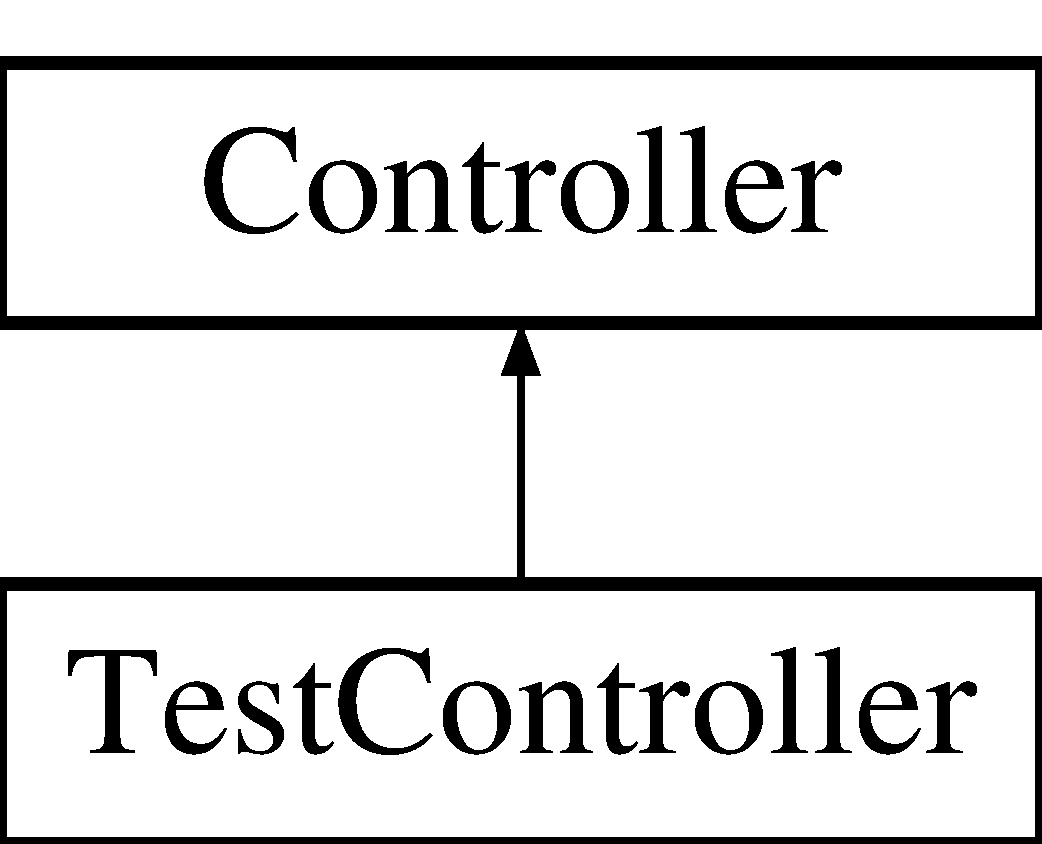
\includegraphics[height=2.000000cm]{class_test_controller}
\end{center}
\end{figure}
\subsection*{Static Public Member Functions}
\begin{DoxyCompactItemize}
\item 
static \hyperlink{class_test_controller_a1f40e85d8731af503764b4098ee17275}{page} (\$p)
\begin{DoxyCompactList}\small\item\em an action called page, shows the action 'page' \item\end{DoxyCompactList}\end{DoxyCompactItemize}


\subsection{Detailed Description}
a typical controller derives from \hyperlink{class_controller}{Controller}. \hyperlink{class_test_controller}{TestController} is a controller named 'test', thus the layout for the controller should be views/layout/test.php, and the views for the actions should be put inside views/test. 

Definition at line 8 of file test\_\-controller.php.



\subsection{Member Function Documentation}
\hypertarget{class_test_controller_a1f40e85d8731af503764b4098ee17275}{
\index{TestController@{TestController}!page@{page}}
\index{page@{page}!TestController@{TestController}}
\subsubsection[{page}]{\setlength{\rightskip}{0pt plus 5cm}static page (
\begin{DoxyParamCaption}
\item[{\$}]{ p}
\end{DoxyParamCaption}
)\hspace{0.3cm}{\ttfamily  \mbox{[}static\mbox{]}}}}
\label{class_test_controller_a1f40e85d8731af503764b4098ee17275}


an action called page, shows the action 'page' 



Definition at line 10 of file test\_\-controller.php.




\begin{DoxyCode}
                          {
    parent::render('test', 'page', $p);
  }
\end{DoxyCode}




The documentation for this class was generated from the following file:\begin{DoxyCompactItemize}
\item 
C:/AppServ/www/book/controllers/\hyperlink{test__controller_8php}{test\_\-controller.php}\end{DoxyCompactItemize}

\chapter{File Documentation}
\hypertarget{controller_8php}{
\section{C:/AppServ/www/book/controller.php File Reference}
\label{controller_8php}\index{C:/AppServ/www/book/controller.php@{C:/AppServ/www/book/controller.php}}
}
\subsection*{Data Structures}
\begin{DoxyCompactItemize}
\item 
class \hyperlink{class_controller}{Controller}
\begin{DoxyCompactList}\small\item\em Defines \hyperlink{class_controller}{Controller} class. \item\end{DoxyCompactList}\end{DoxyCompactItemize}

\hypertarget{test__controller_8php}{
\section{C:/AppServ/www/book/controllers/test\_\-controller.php File Reference}
\label{test__controller_8php}\index{C:/AppServ/www/book/controllers/test\_\-controller.php@{C:/AppServ/www/book/controllers/test\_\-controller.php}}
}
\subsection*{Data Structures}
\begin{DoxyCompactItemize}
\item 
class \hyperlink{class_test_controller}{TestController}
\begin{DoxyCompactList}\small\item\em a typical controller derives from \hyperlink{class_controller}{Controller}. \item\end{DoxyCompactList}\end{DoxyCompactItemize}

\hypertarget{db_8php}{
\section{C:/AppServ/www/book/db.php File Reference}
\label{db_8php}\index{C:/AppServ/www/book/db.php@{C:/AppServ/www/book/db.php}}
}
\subsection*{Data Structures}
\begin{DoxyCompactItemize}
\item 
class \hyperlink{class_database}{Database}
\begin{DoxyCompactList}\small\item\em defines Database(), an interface object providing access to the database. \item\end{DoxyCompactList}\end{DoxyCompactItemize}

\hypertarget{dispatch_8php}{
\section{C:/AppServ/www/book/dispatch.php File Reference}
\label{dispatch_8php}\index{C:/AppServ/www/book/dispatch.php@{C:/AppServ/www/book/dispatch.php}}
}
\subsection*{Data Structures}
\begin{DoxyCompactItemize}
\item 
class \hyperlink{class_dispatcher}{Dispatcher}
\begin{DoxyCompactList}\small\item\em parses the url and invokes the correct controller. \item\end{DoxyCompactList}\end{DoxyCompactItemize}

\hypertarget{index_8php}{
\section{C:/AppServ/www/book/index.php File Reference}
\label{index_8php}\index{C:/AppServ/www/book/index.php@{C:/AppServ/www/book/index.php}}
}

\hypertarget{passwd_8php}{
\section{C:/AppServ/www/book/passwd.php File Reference}
\label{passwd_8php}\index{C:/AppServ/www/book/passwd.php@{C:/AppServ/www/book/passwd.php}}
}
\subsection*{Enumerations}
\begin{DoxyCompactItemize}
\item 
enum \hyperlink{passwd_8php_a8b49cbd6aa98de2ea8630e41f2ba2f71}{DATABASE\_\-URL} 
\begin{DoxyCompactList}\small\item\em contains the passwords to the database. \item\end{DoxyCompactList}\item 
enum \hyperlink{passwd_8php_aa1b72844d2293c7f3c44691cf20a4143}{DATABASE\_\-NAME} 
\item 
enum \hyperlink{passwd_8php_ae355ff3a4a5960b855abdbe2666e5e1d}{USER} 
\item 
enum \hyperlink{passwd_8php_a3326d90c69de890a754f0806f94607e2}{PASSWORD} 
\end{DoxyCompactItemize}


\subsection{Enumeration Type Documentation}
\hypertarget{passwd_8php_aa1b72844d2293c7f3c44691cf20a4143}{
\index{passwd.php@{passwd.php}!DATABASE\_\-NAME@{DATABASE\_\-NAME}}
\index{DATABASE\_\-NAME@{DATABASE\_\-NAME}!passwd.php@{passwd.php}}
\subsubsection[{DATABASE\_\-NAME}]{\setlength{\rightskip}{0pt plus 5cm}enum {\bf DATABASE\_\-NAME}}}
\label{passwd_8php_aa1b72844d2293c7f3c44691cf20a4143}


Definition at line 4 of file passwd.php.

\hypertarget{passwd_8php_a8b49cbd6aa98de2ea8630e41f2ba2f71}{
\index{passwd.php@{passwd.php}!DATABASE\_\-URL@{DATABASE\_\-URL}}
\index{DATABASE\_\-URL@{DATABASE\_\-URL}!passwd.php@{passwd.php}}
\subsubsection[{DATABASE\_\-URL}]{\setlength{\rightskip}{0pt plus 5cm}enum {\bf DATABASE\_\-URL}}}
\label{passwd_8php_a8b49cbd6aa98de2ea8630e41f2ba2f71}


contains the passwords to the database. 



Definition at line 3 of file passwd.php.

\hypertarget{passwd_8php_a3326d90c69de890a754f0806f94607e2}{
\index{passwd.php@{passwd.php}!PASSWORD@{PASSWORD}}
\index{PASSWORD@{PASSWORD}!passwd.php@{passwd.php}}
\subsubsection[{PASSWORD}]{\setlength{\rightskip}{0pt plus 5cm}enum {\bf PASSWORD}}}
\label{passwd_8php_a3326d90c69de890a754f0806f94607e2}


Definition at line 6 of file passwd.php.

\hypertarget{passwd_8php_ae355ff3a4a5960b855abdbe2666e5e1d}{
\index{passwd.php@{passwd.php}!USER@{USER}}
\index{USER@{USER}!passwd.php@{passwd.php}}
\subsubsection[{USER}]{\setlength{\rightskip}{0pt plus 5cm}enum {\bf USER}}}
\label{passwd_8php_ae355ff3a4a5960b855abdbe2666e5e1d}


Definition at line 5 of file passwd.php.


\hypertarget{test_8php}{
\section{C:/AppServ/www/book/views/layouts/test.php File Reference}
\label{test_8php}\index{C:/AppServ/www/book/views/layouts/test.php@{C:/AppServ/www/book/views/layouts/test.php}}
}

\hypertarget{page_8php}{
\section{C:/AppServ/www/book/views/test/page.php File Reference}
\label{page_8php}\index{C:/AppServ/www/book/views/test/page.php@{C:/AppServ/www/book/views/test/page.php}}
}

\printindex
\end{document}
